\fixme{C skal hedde C' i figuren - evt. tilføj $\omega$-vinklen samt navne på
  eksempel bond lengths og bond angles. }
\begin{figure*}
  \centering
  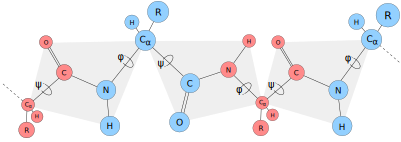
\includegraphics[width=0.75\textwidth]{figures/protein-torsion-angles}
  \caption{}
  \label{fig:protein-torsion-angles}
\end{figure*}

The representation of proteins shown in the structure diagram of
Figure \ref{fig:amino_connect} is suitable for determining the
chemical properties of the molecules, getting an overview of how atoms
are arranged and how the atoms are connected. However, to describe an
exact model of the protein structure we need a lot more precise
characterization. That is, we need to include the concepts of bond
lengths, bond angles and torsional angles into the model. Refer to
Figure \ref{fig:protein-torsion-angles} while reading the following
explanation of these concepts.

\section{Backbone geometry}
\textit{Bond lengths} are the distances between the individual atoms
in a molecule (usually measured in Ångstrøm). We will name the
individual bond lengths by the name of the two atoms which the bond
connects, e.g. the distance between a \Ca\ and N atom in a amino acid
is called \Ca -N. We have computed bond lengths for all bonds in the
backbone, the results are shown in Table
\ref{tab:average_bond_lengths}. As can be seen from the last column in
the table, the variation is very limited and we therefore don't find
it necessary to consider any introduction of variability in these
values.

\begin{table}
  \centering
  \begin{tabular}{lrr}
    \toprule
    Bond & Avg. bond length & Std.dev. \\ \midrule
    C-O   & 1.225998 Å & 0.01883672\\
    CA-C  & 1.527209 Å & 0.01907005\\
    N-CA  & 1.468014 Å & 0.02368912\\
    C-N   & 1.323387 Å & 0.02145554\\
    N-H   & 0.979301 Å & 0.03419159\\
    CA-CB & 1.532714 Å & 0.02276761\\
    CA-HA & 1.074718 Å & 0.03070158\\ \bottomrule
  \end{tabular}
  \vspace{1mm}
  \caption{Average bond lengths (in ångstrøm)}
  \label{tab:average_bond_lengths}
\end{table}

A \textit{bond angle} is an angle between two outgoing bonds from a
single atom. As an example, the angle between the bonds N-\Ca\ and \Ca
-C' is called N-\Ca -C'. Table \ref{tab:average_bond_angles} shows
average values for the backbone bond angles. Again can we see that the
variation is very limited, but as a small displacement can have a
rather large influence it could be considered to introduce the
variability into the model. We have however selected to focus on
the variability in the torsional angles.

\begin{table}
  \centering
  \begin{tabular}{l>{$}r<{^\circ$}>{$}r<{$}}
    \toprule
    \multicolumn{1}{c}{Bond} & \multicolumn{1}{l}{Avg. angle} & \multicolumn{1}{l}{Std.dev.} \\ \midrule 
    H-N-CA & 118.9553 & 1.9979\\
    N-CA-C & 110.6099 & 2.4668\\
    CA-C-O & 120.7088 & 1.3064\\
    CA-C-N & 116.7804 & 1.7682\\
    C-N-CA & 121.4547 & 1.9946\\
    C-N-H  & 119.5112 & 2.1599\\ \bottomrule
  \end{tabular}
  \vspace{1mm}
  \caption{Average bond angles (in degrees)}
  \label{tab:average_bond_angles}
\end{table}

A \textit{torsional angle} is rotational angle around a bond. In the
backbone, there are three of such torsional angles. The $\phi$ and
$\psi$ angles were mentioned earlier. The last one, the $\omega$-angle,
is almost always $0^{\circ}$ and sometimes $180^{\circ}$ according to
\cite{probik}. We will assume that the $\omega$ angle is
\textit{always} $0^{\circ}$. \fixme{or do we assume this?}. To be more
precise the three torsional angles can be defined as dihedral angles
between two planes. For example, the $\phi$ angle can be described by
the angle between the two planes defined by the atoms C'$_{n-1}$,
N$_n$ and \Ca $_n$ as well as N$_n$, \Ca $_n$ and C'$_n$.

\begin{figure*}
	\centering
	\subbottom[]{\includegraphics[width=0.3\textwidth]{figures/ramachandran_except_gly} \label{fig:ramachandran}}
    \subbottom[]{\includegraphics[width=0.3\textwidth]{figures/ramachandran_only_gly} \label{fig:ramachandran_gly}}
    \caption{\textbf{(a)} A ramachandran plot for all amino
      acids except Glycine. \textbf{(b)}  Ramachandran plot
      for Glycine. The plot is adapted from an illustration on Wikipedia, licensed under the Creative Commons Attribution 3.0.}
\end{figure*}



Torsion angles, phi, psi, (omega)
Bond lengths
Bond angles

% As mentioned in our introduction, the largest variability of the
% protein structure is found in the \textit{torsional} angles between
% the individual $C_\alpha$-atoms \cite{lotan04}. These angles are
% termed $\phi$ and $\psi$ in the literature, Figure
% \ref{fig:protein-torsion-agnles} illustrates their definition.

\section{Side-chain geometry}
Rotamers (evt. calculating bond angles and bond lengths)
